\subsection{Verification and Analysis with UPPAAL}
\label{sec:mauppaal}
This section performs a formal analysis of the architectures of water tank. First of all, we encode FMUs of the water tank and model the master algorithm with timed automata. Therefore, the time automata of FMUs and master algorithm compose a network of timed automata. Next, the models are verified with the model checker UPPAAL. 
The execution of FMU and co-simulation is time-related, we have proposed the method to encode FMU with timed automata in Section \ref{sec:encoding}. Here, we abstract the execution of FMUs for the water tank and encode it with the locations and transitions of timed automata. Besides, we also model the master algorithm as a timed automata to coordinate the execution between several FMUs. The timed automata template for FMUs and the master algorithm are shown in Fig.\ref{tk-arch1}. In section \ref{sec:ma}, we have verified three master algorithms. For the case study, we choose rollback algorithm as the master algorithm to coordinate the FMUs. The other two master algorithms can be analysed with the similar way. 

\begin{figure}[htbp]
\centering{
		\subfigure[Timed automata template for FMU controller]{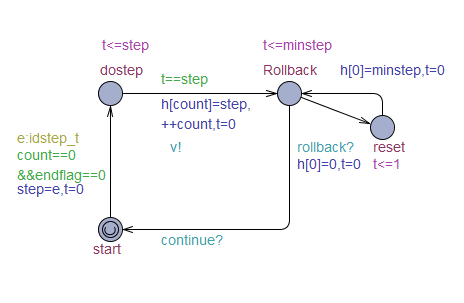
\includegraphics[width=1.6in,height=1.0in]{fig/2signal_controller.png}
			\label{tk_controller}}
		\hfil
		\subfigure[Timed automata for FMU valve]{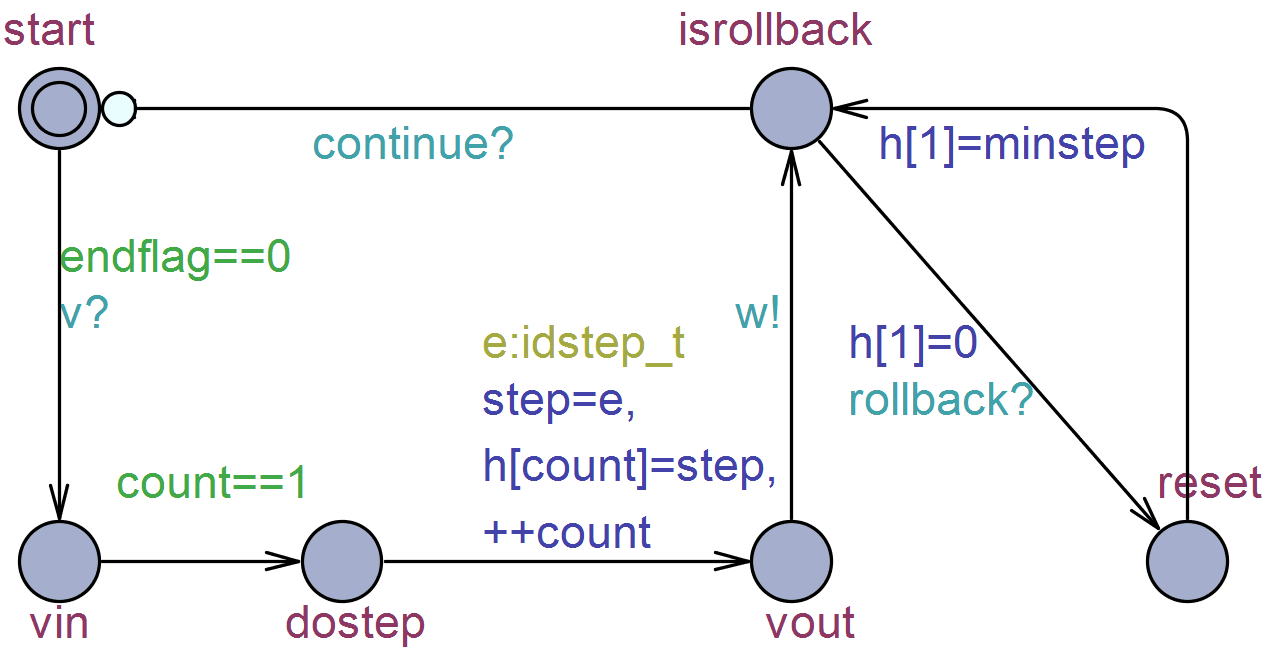
\includegraphics[width=1.6in,height=1.0in]{fig/2signal_v.png}
			\label{tk_v}}
			
	    \subfigure[Timed automata for FMU Water tank1]{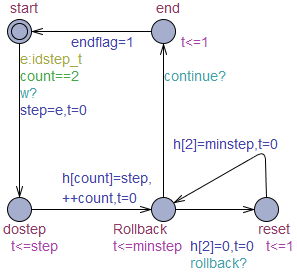
\includegraphics[width=1.5in,height=1.2in]{fig/2signal_wt1.png}
			\label{tk_wt1}}
		\hfil
		 \subfigure[Timed automata for master algorithm]{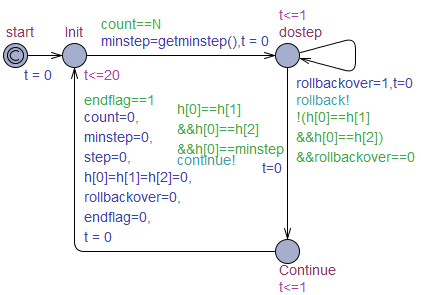
\includegraphics[width=1.7in,height=1.2in]{fig/2signal_master.png}
			\label{tk_ma}}		
	\caption{Network of TA for connection case 1: \emph{TA \_{controller}} $\vert\vert$ \emph{TA \_{valve}} $\vert\vert$ \emph{TA \_{Water tank1}} $\vert\vert$ \emph{TA \_{ma}}.}
	\label{tk-arch1}
	}
\end{figure}

\begin{figure}[htbp]
\centering{
		\subfigure[Execution trace]{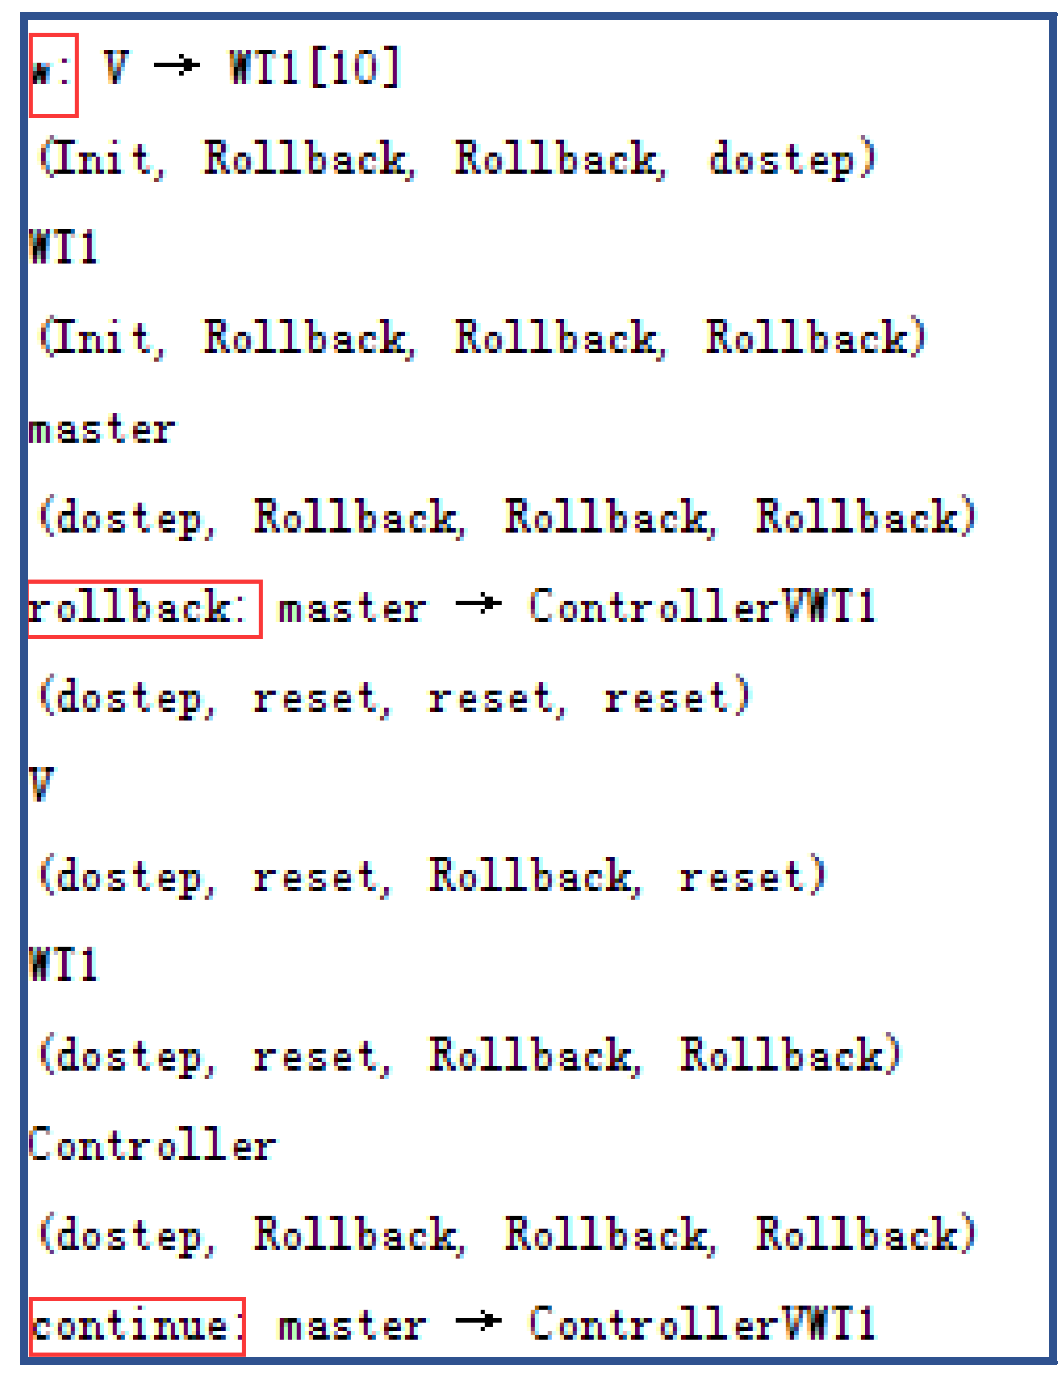
\includegraphics[width=1.6in,height=1.8in]{fig/trs.png}
			\label{trs}}
		\hfil
		\subfigure[Execution sequence diagram]{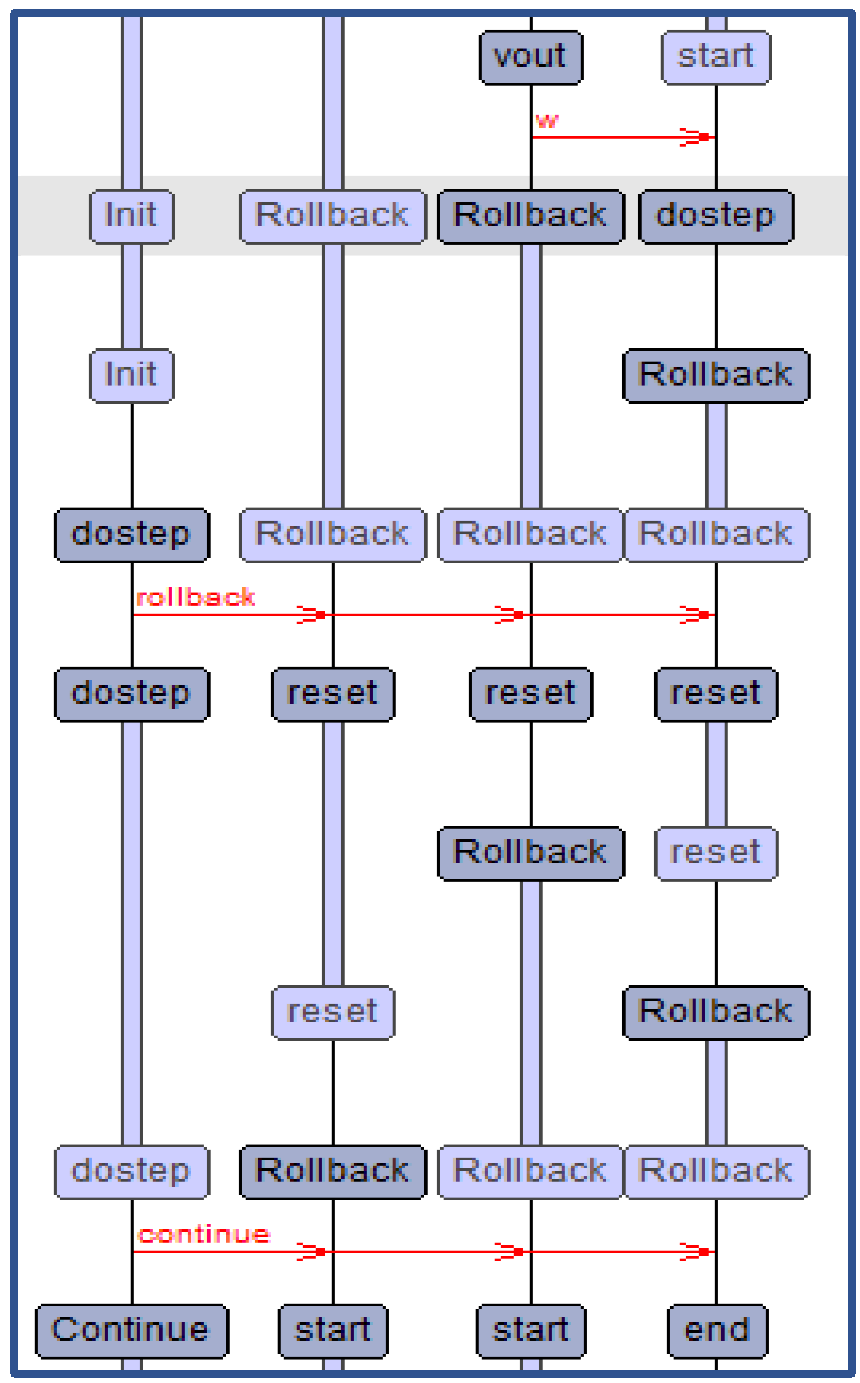
\includegraphics[width=1.6in,height=1.8in]{fig/seq.png}
			\label{seq}}
	\caption{The execution fragment of the co-simulation in UPPAAL.}
	\label{trs-seq}
	}
\end{figure}

Fig.~\ref{tk_controller}, \ref{tk_v}, \ref{tk_wt1} are the templates for \emph{controller}, \emph{valve} and \emph{Water tank1} respectively, they model FMUs of the water tank,  which support rollback function. These FMUs have four key states, e.g., $start$, $dostep$, $Rollback$ and $reset$. Fig.~ \ref{tk_controller} shows the template for \emph{controller} which executes with random step size. It synchronizes with \emph{valve} by signal $v$ and transfers to $Rollback$ state, and then waits for a signal from the master algorithm. Until the \emph{controller} receives the $continue$ signal, it does data exchange with other FMUs, and returns to $start$ state. Otherwise, it receives $rollback$ signal, once it obtains the minimize step size of all FMUs, it transfers to $Rollback$ state. The states and transitions of \emph{valve} and \emph{Water tank1} template are similar with the template of \emph{controller}. Fig.~\ref{tk_ma} shows the template for the master algorithm. Firstly, the master algorithm initializes the parameters, and then it gets minimize step size of FMUs until all FMUs visit $dostep$. Next, the master algorithm decides which signal should be sent according to the guard. If the step sizes of all FMUs are equal, the master algorithm will send $continue$ signal, otherwise, send $rollback$ signal.

Fig.~\ref{trs-seq} is the execution fragment of the co-simulation in UPPAAL, we can find that valve sends a $w$ signal to perform data exchange with \emph{Water tank1}. After that, \emph{Water tank1}  moves to $dostep$ state. The master algorithm sends a $rollback$ signal to all templates, which leads to all of them arrive at $reset$ state. Finally, the master algorithm sends a $continue$ signal to all FMUs. All templates return to $start$ state, and then do the next step. The execution process shows that our models perform correctly.

In order to compare the behavior of three connection cases of water tank system presented in the previous subsection, we also model the other two connection cases in UPPAAL. We add a channel $s$ in the templates for \emph{controller} and \emph{Water tank1} of connection case 1 to model the connection case 2, as shown in Fig.\ref{tk-arch2}. We add a template \emph{Water tank2} and channel $w2$ to model the connection case 3 as shown in Fig.\ref{arc3}. In next subsection, we verify some properties of various connection cases to detect whether there is a loop dependence of the architecture.
\begin{figure}[htbp]
\centering{
		\subfigure[Timed automata for FMU controller]{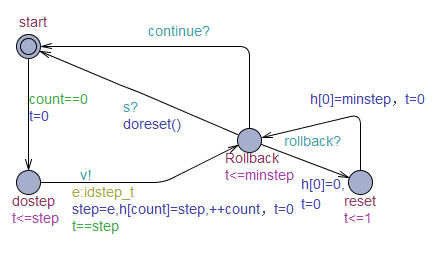
\includegraphics[width=1.8in,height=1.2in]{fig/2signal_cycle_controller.png}
			\label{tk2_controller}}
		\hfil
		\subfigure[Timed automata for FMU Water tank1]{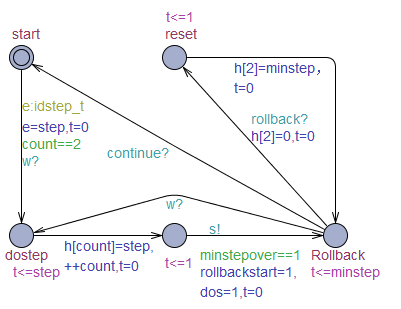
\includegraphics[width=1.5in,height=1.2in]{fig/2signal_cycle_wt1.png}
			\label{tk2_v}}		
	\caption{Network of TA for connection case 2: \emph{TA \_{controller}} $\vert\vert$ \emph{TA \_{valve}} $\vert\vert$ \emph{TA \_{Water tank1}} $\vert\vert$ \emph{TA \_{ma}}.}
	\label{tk-arch2}
	}
\end{figure}
\begin{figure}[htbp]
	\centering	{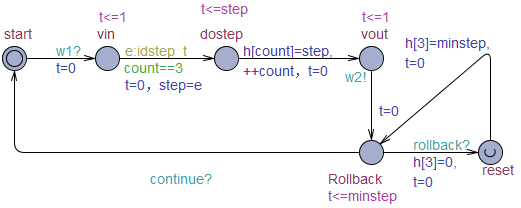
\includegraphics[width=3.5in,height=1.2in]{fig/4signal_wt2.png}}
	\caption{Network of TA for connection case 3: \emph{TA \_{controller}} $\vert\vert$ \emph{TA \_{valve}} $\vert\vert$ \emph{TA \_{Water tank1}} $\vert\vert$ \emph{TA \_{ma}}$\vert\vert$ \emph{TA \_{Water tank1}}.}\label{arc3}
\end{figure}

UPPAAL uses a simplified version of TCTL \cite{BouchenebGR09} to specify the constraint property. We verify the following properties of each connection case:
\begin{itemize}
\item
$E\langle\rangle~WT1.Rollback$ and $E\langle\rangle~master.Continue$ are reachability properties checking whether FMU of \emph{Water tank1} can reach $Rollback$ state and whether the master algorithm can reach $Continue$ state respectively.
\item
$master.start \rightarrow master.Continue$ are liveness property. If the master algorithm arrive at $start$ state, it eventually reaches $Continue$ state.
\item 
$A[]~not~deadlock$ is safety property checking whether the model will be deadlock.
\end{itemize}

The verification results are listed in Table \ref{rs}. We can find that all properties of connection case 1 and 3 are satisfied. It shows that our master algorithm works well and the composition of FMUs is determinate. However, the liveness and reachability properties of connection case 2 are not satisfied. We find that there is an algebraic loop which may be introduced with the I/O dependency in this connection case. The experimental results show that our approach is feasible and useful for model checking the FMI co-simulation.
Here, we only focus on the detection of algebraic loop and the correctness of co-simulation. In the future work, we will consider eliminating the algebraic loop.  
\begin{table}
\caption{Experimental results for various connection case}
\centering
\begin{tabular}{c c c} 
        \hline  
        Connection case & Property & Result\\
        \hline
        \multirow{2}{2.0cm}{Case 1}  
                & $E\langle\rangle~WT1.Rollback$ & True\\ 
                & $E\langle\rangle~master.Continue$ & True\\ 
                & $master.start\rightarrow master.Continue$ & True\\ 
                & $A[]~not~deadlock$ & True\\   
        \hline 
        \multirow{2}{2.0cm}{Case 2}  
                & $E\langle\rangle~WT1.Rollback$ & True\\ 
                & $E\langle\rangle~master.Continue$ & False\\ 
                & $master.start\rightarrow master.Continue$ & False\\ 
                & $A[]~not~deadlock$ & True\\   
        \hline 
        \multirow{2}{2.0cm}{Case 3}  
                & $E\langle\rangle~WT1.Rollback$ & True\\ 
                & $E\langle\rangle~master.Continue$ & True\\ 
                & $master.start \rightarrow master.Continue$ & True\\ 
                & $A[]~not~deadlock$ & True\\   
        \hline 
\end{tabular} 
\label{rs}
\end{table}




